\documentclass[10pt,a4paper]{article}

% Packages
\usepackage{fancyhdr}           % For header and footer
\usepackage{multicol}           % Allows multicols in tables
\usepackage{tabularx}           % Intelligent column widths
\usepackage{tabulary}           % Used in header and footer
\usepackage{hhline}             % Border under tables
\usepackage{graphicx}           % For images
\usepackage{xcolor}             % For hex colours
%\usepackage[utf8x]{inputenc}    % For unicode character support
\usepackage[T1]{fontenc}        % Without this we get weird character replacements
\usepackage{colortbl}           % For coloured tables
\usepackage{setspace}           % For line height
\usepackage{lastpage}           % Needed for total page number
\usepackage{seqsplit}           % Splits long words.
%\usepackage{opensans}          % Can't make this work so far. Shame. Would be lovely.
\usepackage[normalem]{ulem}     % For underlining links
% Most of the following are not required for the majority
% of cheat sheets but are needed for some symbol support.
\usepackage{amsmath}            % Symbols
\usepackage{MnSymbol}           % Symbols
\usepackage{wasysym}            % Symbols
%\usepackage[english,german,french,spanish,italian]{babel} % Languages

% Lengths and widths
\addtolength{\textwidth}{6cm}
\addtolength{\textheight}{-1cm}
\addtolength{\hoffset}{-3cm}
\addtolength{\voffset}{-2cm}
\setlength{\tabcolsep}{0.2cm} % Space between columns
\setlength{\headsep}{-12pt} % Reduce space between header and content
\setlength{\headheight}{50pt} % If less, LaTeX automatically increases it
\renewcommand{\footrulewidth}{0pt} % Remove footer line
\renewcommand{\headrulewidth}{0pt} % Remove header line
\renewcommand{\seqinsert}{\ifmmode\allowbreak\else\-\fi} % Hyphens in seqsplit
% This two commands together give roughly
% the right line height in the tables
\renewcommand{\arraystretch}{1.3}
\onehalfspacing

% Commands
\newcommand{\SetRowColor}[1]{\noalign{\gdef\RowColorName{#1}}\rowcolor{\RowColorName}} % Shortcut for row colour
\newcommand{\mymulticolumn}[3]{\multicolumn{#1}{>{\columncolor{\RowColorName}}#2}{#3}} % For coloured multi-cols
\newcolumntype{x}[1]{>{\raggedright}p{#1}} % New column types for ragged-right paragraph columns
\newcommand{\tn}{\tabularnewline} % Required as custom column type in use

% Font and Colours
\definecolor{HeadBackground}{HTML}{333333}
\definecolor{FootBackground}{HTML}{666666}
\definecolor{TextColor}{HTML}{333333}
\definecolor{DarkBackground}{HTML}{009AC4}
\definecolor{TitleBackground}{HTML}{0289A8}
\definecolor{LightBackground}{HTML}{BADCE4}
\renewcommand{\familydefault}{\sfdefault}
\color{TextColor}

% Header and Footer
\pagestyle{fancy}
\fancyhead{} % Set header to blank
\fancyfoot{} % Set footer to blank
\fancyhead[L]{
\noindent
\begin{multicols}{1}
\begin{tabulary}{5cm}{L}
    \vspace{-2pt}\large{\bf{\textcolor{DarkBackground}{\textrm{Git Cheat Sheet}}}} \\
\end{tabulary}
\end{multicols}}

\begin{document}
	\raggedright
	\raggedcolumns
	\footnotesize
	\begin{multicols*}{3}
	
		% Command
		\begin{tabularx}{5.377cm}{X}
			\SetRowColor{DarkBackground}
			\mymulticolumn{1}{x{5.377cm}}{\bf\textcolor{white}{Command}}  \tn
			
			\SetRowColor{TitleBackground}
			\mymulticolumn{1}{x{5.377cm}}{\bf{Observe your Repository}} \tn
			
			\SetRowColor{LightBackground}
			\mymulticolumn{1}{x{5.377cm}}{{\bf{List new or modified files not yet
			committed}}} \tn
			\SetRowColor{white}
			\mymulticolumn{1}{x{5.377cm}}{{\textcolor{red}{g}it \textcolor{red}{s}ta\textcolor{red}{t}us}} \tn
			
			\SetRowColor{LightBackground}
			\mymulticolumn{1}{x{5.377cm}}{{\bf{Show the changes to files not yet staged}}} \tn
			\SetRowColor{white}
			\mymulticolumn{1}{x{5.377cm}}{{\textcolor{red}{g}it \textcolor{red}{d}iff}} \tn
			
			\SetRowColor{LightBackground}
			\mymulticolumn{1}{x{5.377cm}}{{\bf{Show full change history}}} \tn
			\SetRowColor{white}
			\mymulticolumn{1}{x{5.377cm}}{{\textcolor{red}{g}it \textcolor{red}{l}og}} \tn
		\end{tabularx}
		
		\begin{tabularx}{5.377cm}{X}
			\SetRowColor{TitleBackground}
			\mymulticolumn{1}{x{5.377cm}}{\bf{Synchronize}} \tn
			
			\SetRowColor{LightBackground}
			\mymulticolumn{1}{x{5.377cm}}{{\bf{Get the latest changes from origin
			(no merge)}}} \tn
			\SetRowColor{white}
			\mymulticolumn{1}{x{5.377cm}}{{\textcolor{red}{g}it \textcolor{red}{fetch}}} \tn
			
			\SetRowColor{LightBackground}
			\mymulticolumn{1}{x{5.377cm}}{{\bf{Fetch the latest changes from origin
			and merge}}} \tn
			\SetRowColor{white}
			\mymulticolumn{1}{x{5.377cm}}{{\textcolor{red}{g}it \textcolor{red}{pull}}} \tn
			
			\SetRowColor{LightBackground}
			\mymulticolumn{1}{x{5.377cm}}{{\bf{Fetch the latest changes from origin
			and rebase}}} \tn
			\SetRowColor{white}
			\mymulticolumn{1}{x{5.377cm}}{{\textcolor{red}{g}it \textcolor{red}{pull} --\textcolor{red}{r}ebase}} \tn
			
			\SetRowColor{LightBackground}
			\mymulticolumn{1}{x{5.377cm}}{{\bf{Push local changes to the origin}}} \tn
			\SetRowColor{white}
			\mymulticolumn{1}{x{5.377cm}}{{\textcolor{red}{g}it \textcolor{red}{push}}} \tn
		\end{tabularx}
		
		\begin{tabularx}{5.377cm}{X}
		
			\SetRowColor{TitleBackground}
			\mymulticolumn{1}{x{5.377cm}}{\bf{Working with Branches}} \tn
			
			\SetRowColor{LightBackground}
			\mymulticolumn{1}{x{5.377cm}}{{\bf{List all local branches }}} \tn
			\SetRowColor{white}
			\mymulticolumn{1}{x{5.377cm}}{{\textcolor{red}{g}it \textcolor{red}{b}ranch}} \tn
			
			\SetRowColor{LightBackground}
			\mymulticolumn{1}{x{5.377cm}}{{\bf{List all branches, local and remote}}} \tn
			\SetRowColor{white}
			\mymulticolumn{1}{x{5.377cm}}{{\textcolor{red}{g}it \textcolor{red}{b}ranch -av}} \tn
			
			\SetRowColor{LightBackground}
			\mymulticolumn{1}{x{5.377cm}}{{\bf{Create a new branch called my-branch}}} \tn
			\SetRowColor{white}
			\mymulticolumn{1}{x{5.377cm}}{{\textcolor{red}{g}it \textcolor{red}{b}ranch \emph{my-branch}}} \tn
			
			\SetRowColor{LightBackground}
			\mymulticolumn{1}{x{5.377cm}}{{\bf{Switch to a branch and update working directory}}} \tn
			\SetRowColor{white}
			\mymulticolumn{1}{x{5.377cm}}{{\textcolor{red}{g}it \textcolor{red}{c}heck\textcolor{red}{o}ut \emph{branch-name}}} \tn
			
			\SetRowColor{LightBackground}
			\mymulticolumn{1}{x{5.377cm}}{{\bf{Delete the branch called my-branch}}} \tn
			\SetRowColor{white}
			\mymulticolumn{1}{x{5.377cm}}{{\textcolor{red}{g}it \textcolor{red}{b}ranch -d \emph{my-branch}}} \tn
			
			\SetRowColor{LightBackground}
			\mymulticolumn{1}{x{5.377cm}}{{\bf{Merge branch-a into branch-b}}} \tn
			\SetRowColor{white}
			\mymulticolumn{1}{x{5.377cm}}{{\textcolor{red}{g}it \textcolor{red}{c}heck\textcolor{red}{o}ut \emph{branch-b}}} \tn
			\SetRowColor{white}
			\mymulticolumn{1}{x{5.377cm}}{{\textcolor{red}{g}it \textcolor{red}{m}erge \emph{branch-a}}} \tn
			
			\SetRowColor{LightBackground}
			\mymulticolumn{1}{x{5.377cm}}{{\bf{Tag the current commit}}} \tn
			\SetRowColor{white}
			\mymulticolumn{1}{x{5.377cm}}{{ git tag my-tag}} \tn
		\end{tabularx}
		
		\begin{tabularx}{5.377cm}{X}
			\SetRowColor{TitleBackground}
			\mymulticolumn{1}{x{5.377cm}}{\bf{Make a change}} \tn
			
			\SetRowColor{LightBackground}
			\mymulticolumn{1}{x{5.377cm}}{{\bf{Stages the file, ready for commit}}} \tn
			\SetRowColor{white}
			\mymulticolumn{1}{x{5.377cm}}{{\textcolor{red}{g}it \textcolor{red}{a}dd [file]}} \tn
			
			\SetRowColor{LightBackground}
			\mymulticolumn{1}{x{5.377cm}}{{\bf{Commit all staged files to versioned history}}} \tn
			\SetRowColor{white}
			\mymulticolumn{1}{x{5.377cm}}{{\textcolor{red}{g}it \textcolor{red}{c}ommit -\textcolor{red}{m} "commit message"}} \tn
			
			\SetRowColor{LightBackground}
			\mymulticolumn{1}{x{5.377cm}}{{\bf{Unstages file, keeping the file changes}}} \tn
			\SetRowColor{white}
			\mymulticolumn{1}{x{5.377cm}}{{\textcolor{red}{g}it \textcolor{red}{r}eset [file]}} \tn
			
			\SetRowColor{LightBackground}
			\mymulticolumn{1}{x{5.377cm}}{{\bf{Undoes all commits afer [commit], preserving change locally}}} \tn
			\SetRowColor{white}
			\mymulticolumn{1}{x{5.377cm}}{{\textcolor{red}{g}it \textcolor{red}{r}eset [commit]}} \tn
			
			\SetRowColor{LightBackground}
			\mymulticolumn{1}{x{5.377cm}}{{\bf{Discards all history and changes back to the specified commit}}} \tn
			\SetRowColor{white}
			\mymulticolumn{1}{x{5.377cm}}{{\textcolor{red}{g}it \textcolor{red}{r}eset --hard [commit]}} \tn
		\end{tabularx}
		
		
		\begin{tabularx}{5.377cm}{X}
			\SetRowColor{TitleBackground}
			\mymulticolumn{1}{x{5.377cm}}{\bf{Save fragments}} \tn
			
			\SetRowColor{LightBackground}
			\mymulticolumn{1}{x{5.377cm}}{{\bf{Lists all stashed changesets}}} \tn
			\SetRowColor{white}
			\mymulticolumn{1}{x{5.377cm}}{{\textcolor{red}{g}it \textcolor{red}{stash l}ist}} \tn
			
			\SetRowColor{LightBackground}
			\mymulticolumn{1}{x{5.377cm}}{{\bf{Temporarily stores all modified tracked files}}} \tn
			\SetRowColor{white}
			\mymulticolumn{1}{x{5.377cm}}{{\textcolor{red}{g}it \textcolor{red}{stash}}} \tn
			
			\SetRowColor{LightBackground}
			\mymulticolumn{1}{x{5.377cm}}{{\bf{Temporarily stores all modified tracked files with a stash name}}} \tn
			\SetRowColor{white}
			\mymulticolumn{1}{x{5.377cm}}{{\textcolor{red}{g}it \textcolor{red}{stash s}a\textcolor{red}{v}e "stash-name"}} \tn
			
			\SetRowColor{LightBackground}
			\mymulticolumn{1}{x{5.377cm}}{{\bf{Details stash number 'n'}}} \tn
			\SetRowColor{white}
			\mymulticolumn{1}{x{5.377cm}}{{\textcolor{red}{g}it \textcolor{red}{stash sh}ow stash@\{n\} -p}} \tn
			
			\SetRowColor{LightBackground}
			\mymulticolumn{1}{x{5.377cm}}{{\bf{Restores stash  number 'n'}}} \tn
			\SetRowColor{white}
			\mymulticolumn{1}{x{5.377cm}}{{\textcolor{red}{g}it \textcolor{red}{stash a}pply stash@\{n\}}} \tn
			
			\SetRowColor{LightBackground}
			\mymulticolumn{1}{x{5.377cm}}{{\bf{Discards stash  number 'n'}}} \tn
			\SetRowColor{white}
			\mymulticolumn{1}{x{5.377cm}}{{\textcolor{red}{g}it \textcolor{red}{stash d}rop stash@\{n\}}} \tn
			
			\SetRowColor{LightBackground}
			\mymulticolumn{1}{x{5.377cm}}{{\bf{Restores the most recently stashed files }}} \tn
			\SetRowColor{white}
			\mymulticolumn{1}{x{5.377cm}}{{\textcolor{red}{g}it \textcolor{red}{stash p}op}} \tn
			
			\hhline{>{\arrayrulecolor{DarkBackground}}-}
		\end{tabularx}
		
			\par\addvspace{1.3em}
		
		\begin{tabularx}{5.377cm}{X}
			\SetRowColor{DarkBackground}
			\mymulticolumn{1}{x{5.377cm}}{\bf\textcolor{white}{Oh Shit, Git!}}  \tn
			
			\SetRowColor{LightBackground}
			\mymulticolumn{1}{x{5.377cm}}{{\bf{I did something terribly wrong, please tell me git has a magic time machine!?!}}} \tn
			\SetRowColor{white}
			\mymulticolumn{1}{x{5.377cm}}{{\textcolor{red}{g}it \textcolor{red}{r}ef\textcolor{red}{l}og}} \tn
			\mymulticolumn{1}{x{5.377cm}}{{\emph{
			\# you will see a list of every thing you've done in git, across all branches! \\
			\# each one has an index HEAD@\{index\} \\
			\# find the one before you broke everything}}} \tn
			\mymulticolumn{1}{x{5.377cm}}{{\textcolor{red}{g}it \textcolor{red}{r}eset HEAD@\{index\}}} \tn
			\mymulticolumn{1}{x{5.377cm}}{{\emph{\# magic time machine}}} \tn
			
			\SetRowColor{LightBackground}
			\mymulticolumn{1}{x{5.377cm}}{{\bf{I committed and immediately realized I need to make one small change!}}} \tn
			\SetRowColor{white}
			\mymulticolumn{1}{x{5.377cm}}{{\emph{\# make your change}}} \tn
			\mymulticolumn{1}{x{5.377cm}}{{\textcolor{red}{g}it \textcolor{red}{a}dd . \# or add individual files}} \tn
			\mymulticolumn{1}{x{5.377cm}}{{\textcolor{red}{g}it \textcolor{red}{c}ommit --\textcolor{red}{a}mend }} \tn
			\mymulticolumn{1}{x{5.377cm}}{{\emph{\# follow prompts to change or keep the commit message \\
			\# now your last commit contains that change!}}} \tn
			
			\SetRowColor{LightBackground}
			\mymulticolumn{1}{x{5.377cm}}{{\bf{I need to change the message on my last commit!}}} \tn
			\SetRowColor{white}
			\mymulticolumn{1}{x{5.377cm}}{{\textcolor{red}{g}it \textcolor{red}{c}ommit --\textcolor{red}{a}mend }} \tn
			\mymulticolumn{1}{x{5.377cm}}{{\emph{\# follow prompts to change or keep the commit message}}} \tn
			
			\SetRowColor{LightBackground}
			\mymulticolumn{1}{x{5.377cm}}{{\bf{I accidentally committed something to master that should have been on a brand new branch!}}} \tn
			\SetRowColor{white}
			\mymulticolumn{1}{x{5.377cm}}{{\emph{\# create a new branch from the current state of master}}} \tn
			\mymulticolumn{1}{x{5.377cm}}{{\textcolor{red}{g}it \textcolor{red}{b}ranch \emph{branch-name}}} \tn
			\mymulticolumn{1}{x{5.377cm}}{{\emph{\# remove the commit from the master branch}}} \tn
			\mymulticolumn{1}{x{5.377cm}}{{\textcolor{red}{g}it \textcolor{red}{r}eset HEAD\~ --hard }} \tn
			\mymulticolumn{1}{x{5.377cm}}{{\textcolor{red}{g}it \textcolor{red}{c}heckout \emph{branch-name}}} \tn
			\mymulticolumn{1}{x{5.377cm}}{{\emph{\# your commit lives in this branch now}}} \tn
			
			\SetRowColor{LightBackground}
			\mymulticolumn{1}{x{5.377cm}}{{\bf{I accidentally committed to the wrong branch!}}} \tn
			\SetRowColor{white}
			\mymulticolumn{1}{x{5.377cm}}{{\emph{\# undo the last commit, but leave the changes available}}} \tn
			\mymulticolumn{1}{x{5.377cm}}{{\textcolor{red}{g}it \textcolor{red}{r}eset HEAD\~ --soft}} \tn
			\mymulticolumn{1}{x{5.377cm}}{{\textcolor{red}{g}it \textcolor{red}{stash}}} \tn
			\mymulticolumn{1}{x{5.377cm}}{{\emph{\# move to the correct branch}}} \tn
			\mymulticolumn{1}{x{5.377cm}}{{\textcolor{red}{g}it \textcolor{red}{c}heckout \emph{branch-name}}} \tn
			\mymulticolumn{1}{x{5.377cm}}{{\textcolor{red}{g}it \textcolor{red}{stash p}op}} \tn
			\mymulticolumn{1}{x{5.377cm}}{{\textcolor{red}{g}it \textcolor{red}{a}dd . \emph{\# or add individual files}}} \tn
			\mymulticolumn{1}{x{5.377cm}}{{\textcolor{red}{g}it \textcolor{red}{c}ommit -\textcolor{red}{m} "your message here" }} \tn
			\mymulticolumn{1}{x{5.377cm}}{{\emph{\# now your changes are on the correct branch}}} \tn
			\hhline{>{\arrayrulecolor{DarkBackground}}-}
		\end{tabularx}
		
			\par\addvspace{1.3em}
		
		% FEATURE FLOW
		\begin{tabularx}{5.377cm}{X}
			\SetRowColor{DarkBackground}
			\mymulticolumn{1}{x{5.377cm}}{\bf\textcolor{white}{Feature Flow}}  \tn
			
			\SetRowColor{LightBackground}
			\mymulticolumn{1}{p{5.377cm}}{\vspace{1px}\centerline{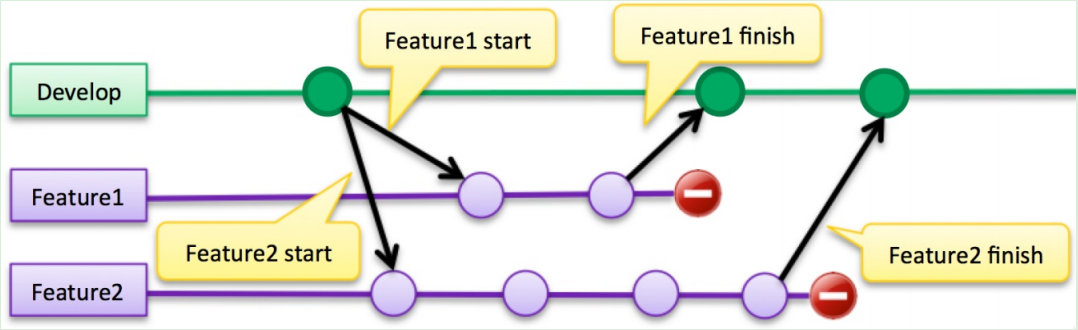
\includegraphics[width=5.1cm]{feature.PNG}}} \tn
			\hhline{>{\arrayrulecolor{DarkBackground}}-}
			
			\SetRowColor{TitleBackground}
			\mymulticolumn{1}{x{5.377cm}}{\bf{Feature start}} \tn
			
			\SetRowColor{white}
			\mymulticolumn{1}{x{5.377cm}}{{\textcolor{red}{g}it \textcolor{red}{c}heck\textcolor{red}{o}ut develop}} \tn
			
			\SetRowColor{LightBackground}
			\mymulticolumn{1}{x{5.377cm}}{{\textcolor{red}{g}it \textcolor{red}{pull} --\textcolor{red}{r}ebase origin develop}} \tn
		
				\SetRowColor{white}
			\mymulticolumn{1}{x{5.377cm}}{{\textcolor{red}{g}it \textcolor{red}{c}heck\textcolor{red}{o}ut  -b feature/{\emph{nomfeature}}}} \tn
		
				\SetRowColor{TitleBackground}
			\mymulticolumn{1}{x{5.377cm}}{\bf{Feature Share}} \tn
			\SetRowColor{LightBackground}
			\mymulticolumn{1}{x{5.377cm}}{{\textcolor{red}{g}it \textcolor{red}{push} origin feature/\emph{nomfeature}}} \tn
		
				\SetRowColor{TitleBackground}
			\mymulticolumn{1}{x{5.377cm}}{\bf{Feature finish}} \tn
		
				\SetRowColor{LightBackground}
			\mymulticolumn{1}{x{5.377cm}}{{\textcolor{red}{g}it \textcolor{red}{c}heck\textcolor{red}{o}ut develop}} \tn
		
				\SetRowColor{white}
			\mymulticolumn{1}{x{5.377cm}}{{\textcolor{red}{g}it \textcolor{red}{m}erge --\textcolor{red}{no}-\textcolor{red}{ff} feature/{\emph{nomefeature}}}} \tn
		
				\SetRowColor{LightBackground}
			\mymulticolumn{1}{x{5.377cm}}{{\textcolor{red}{g}it \textcolor{red}{b}ranch -d feature/{\emph{nomefeature}}}} \tn
		
				\SetRowColor{white}
			\mymulticolumn{1}{x{5.377cm}}{{\textcolor{red}{g}it \textcolor{red}{push} origin develop}} \tn
		
				\SetRowColor{LightBackground}
			\mymulticolumn{1}{x{5.377cm}}{{\textcolor{red}{g}it \textcolor{red}{push} origin :feature/{\emph{nomefeature}} (if pushed)}} \tn
			\hhline{>{\arrayrulecolor{DarkBackground}}-}
		\end{tabularx}
		\par\addvspace{1.3em}
		
		\begin{tabularx}{5.377cm}{X}
			\SetRowColor{DarkBackground}
			\mymulticolumn{1}{x{5.377cm}}{\bf\textcolor{white}{Hotfix Flow}}  \tn
			\SetRowColor{LightBackground}
			\mymulticolumn{1}{p{5.377cm}}{\vspace{1px}\centerline{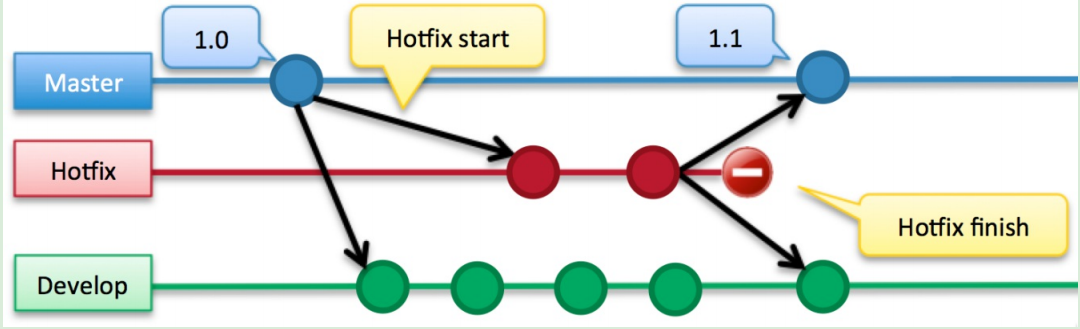
\includegraphics[width=5.1cm]{hotfix.PNG}}} \tn
			\hhline{>{\arrayrulecolor{DarkBackground}}-}
			
			\SetRowColor{TitleBackground}
			\mymulticolumn{1}{x{5.377cm}}{\bf{Hotfix start}} \tn
			
			\SetRowColor{white}
			\mymulticolumn{1}{x{5.377cm}}{{\textcolor{red}{g}it \textcolor{red}{c}heck\textcolor{red}{o}ut develop}} \tn
			
			\SetRowColor{LightBackground}
			\mymulticolumn{1}{x{5.377cm}}{{\textcolor{red}{g}it \textcolor{red}{pull} --\textcolor{red}{r}ebase origin develop}} \tn
			
			\SetRowColor{white}
			\mymulticolumn{1}{x{5.377cm}}{{\textcolor{red}{g}it \textcolor{red}{c}heck\textcolor{red}{o}ut -b hotfix/{\emph{hotfix-version}} }} \tn
			
			\SetRowColor{TitleBackground}
			\mymulticolumn{1}{x{5.377cm}}{\bf{Hotfix finish}} \tn
			
			\SetRowColor{LightBackground}
			\mymulticolumn{1}{x{5.377cm}}{\textcolor{red}{g}it \textcolor{red}{c}heck\textcolor{red}{o}ut master} \tn
			
			\SetRowColor{white}
			\mymulticolumn{1}{x{5.377cm}}{{\textcolor{red}{g}it \textcolor{red}{m}erge --\textcolor{red}{no}-\textcolor{red}{ff} hotfix/\emph{hotfix-version}}} \tn
			
			\SetRowColor{LightBackground}
			\mymulticolumn{1}{x{5.377cm}}{{git tag -a {\emph{hotfix-version}} }} \tn
			
			\SetRowColor{white}
			\mymulticolumn{1}{x{5.377cm}}{{\textcolor{red}{g}it \textcolor{red}{c}heck\textcolor{red}{o}ut develop}} \tn
			
			\SetRowColor{LightBackground}
			\mymulticolumn{1}{x{5.377cm}}{{\textcolor{red}{g}it \textcolor{red}{m}erge --\textcolor{red}{no}-\textcolor{red}{ff} hotfix/\emph{hotfix-version}}} \tn
			
			\SetRowColor{LightBackground}
			\mymulticolumn{1}{x{5.377cm}}{{\textcolor{red}{g}it \textcolor{red}{b}ranch -d hotfix/\emph{hotfix-version}}} \tn
			
			\SetRowColor{white}
			\mymulticolumn{1}{x{5.377cm}}{{\textcolor{red}{g}it \textcolor{red}{push} origin master}} \tn
			
			\SetRowColor{LightBackground}
			\mymulticolumn{1}{x{5.377cm}}{{\textcolor{red}{g}it \textcolor{red}{push} origin develop}} \tn
			
			\SetRowColor{white}
			\mymulticolumn{1}{x{5.377cm}}{{\textcolor{red}{g}it \textcolor{red}{push} origin --tags}} \tn
			
			\SetRowColor{LightBackground}
			\mymulticolumn{1}{x{5.377cm}}{{\textcolor{red}{g}it \textcolor{red}{push} origin :hotfix/\emph{hotfix-version} (if pushed)}} \tn
		
				\hhline{>{\arrayrulecolor{DarkBackground}}-}
		\end{tabularx}
		\par\addvspace{1.3em}
		
		
		% RELEASE
		\begin{tabularx}{5.377cm}{X}
			\SetRowColor{DarkBackground}
			\mymulticolumn{1}{x{5.377cm}}{\bf\textcolor{white}{Release Flow}}  \tn
			\SetRowColor{LightBackground}
			\mymulticolumn{1}{p{5.377cm}}{\vspace{1px}\centerline{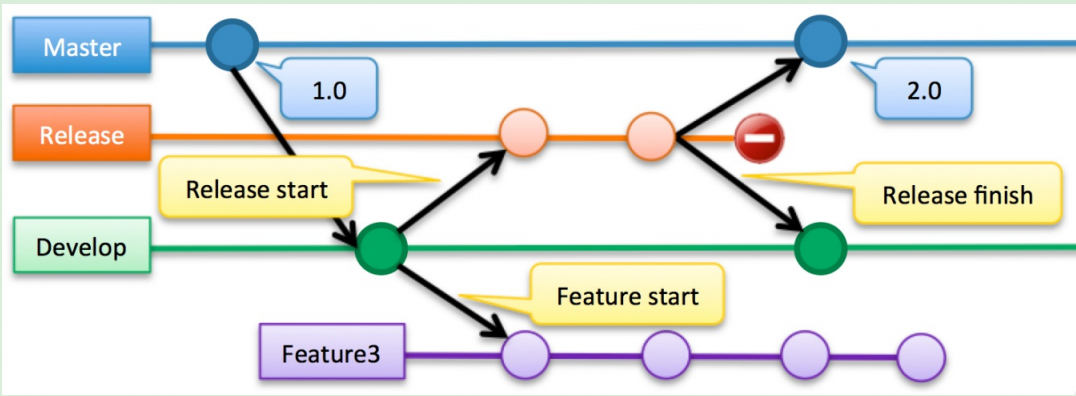
\includegraphics[width=5.1cm]{release.PNG}}} \tn
			\hhline{>{\arrayrulecolor{DarkBackground}}-}
			
			\SetRowColor{TitleBackground}
			\mymulticolumn{1}{x{5.377cm}}{\bf{Release start}} \tn
			
			\SetRowColor{white}
			\mymulticolumn{1}{x{5.377cm}}{{\textcolor{red}{g}it \textcolor{red}{c}heck\textcolor{red}{o}ut develop}} \tn
			
			\SetRowColor{LightBackground}
			\mymulticolumn{1}{x{5.377cm}}{{\textcolor{red}{g}it \textcolor{red}{pull} --\textcolor{red}{r}ebase origin develop}} \tn
			
			\SetRowColor{white}
			\mymulticolumn{1}{x{5.377cm}}{{\textcolor{red}{g}it \textcolor{red}{c}heck\textcolor{red}{o}ut -b release/{\emph{release-version}} }} \tn
			
			\SetRowColor{TitleBackground}
			\mymulticolumn{1}{x{5.377cm}}{\bf{Release Share}} \tn
			\SetRowColor{LightBackground}
			\mymulticolumn{1}{x{5.377cm}}{{\textcolor{red}{g}it \textcolor{red}{push} origin feature/\emph{release-version}}} \tn
			
			
			\SetRowColor{TitleBackground}
			\mymulticolumn{1}{x{5.377cm}}{\bf{Release finish}} \tn
			
			\SetRowColor{LightBackground}
			\mymulticolumn{1}{x{5.377cm}}{\textcolor{red}{g}it \textcolor{red}{c}heck\textcolor{red}{o}ut master} \tn
			
			\SetRowColor{white}
			\mymulticolumn{1}{x{5.377cm}}{{\textcolor{red}{g}it \textcolor{red}{m}erge --\textcolor{red}{no}-\textcolor{red}{ff} release/\emph{release-version}}} \tn
			
			\SetRowColor{LightBackground}
			\mymulticolumn{1}{x{5.377cm}}{{git tag -a {\emph{release-version}} }} \tn
			
			\SetRowColor{white}
			\mymulticolumn{1}{x{5.377cm}}{{\textcolor{red}{g}it \textcolor{red}{c}heck\textcolor{red}{o}ut develop}} \tn
			
			\SetRowColor{LightBackground}
			\mymulticolumn{1}{x{5.377cm}}{{\textcolor{red}{g}it \textcolor{red}{m}erge --\textcolor{red}{no}-\textcolor{red}{ff} release/\emph{release-version}}} \tn
			
			\SetRowColor{LightBackground}
			\mymulticolumn{1}{x{5.377cm}}{{\textcolor{red}{g}it \textcolor{red}{b}ranch -d release/\emph{release-version}}} \tn
			
			\SetRowColor{white}
			\mymulticolumn{1}{x{5.377cm}}{{\textcolor{red}{g}it \textcolor{red}{push} origin master}} \tn
			
			\SetRowColor{LightBackground}
			\mymulticolumn{1}{x{5.377cm}}{{\textcolor{red}{g}it \textcolor{red}{push} origin develop}} \tn
			
			\SetRowColor{white}
			\mymulticolumn{1}{x{5.377cm}}{{\textcolor{red}{g}it \textcolor{red}{push} origin --tags}} \tn
			
			\SetRowColor{LightBackground}
			\mymulticolumn{1}{x{5.377cm}}{{\textcolor{red}{g}it \textcolor{red}{push} origin :release/\emph{release-version} (if pushed)}} \tn
		\end{tabularx}
		\par\addvspace{1.3em}
		
	\end{multicols*}

\end{document}
